\section{Results and Discussion}

\subsection{Study 1: The Impact of Estimator Choice and Sample Size on Model Evaluation Reliability}

\begin{figure}[H]
    \centering
    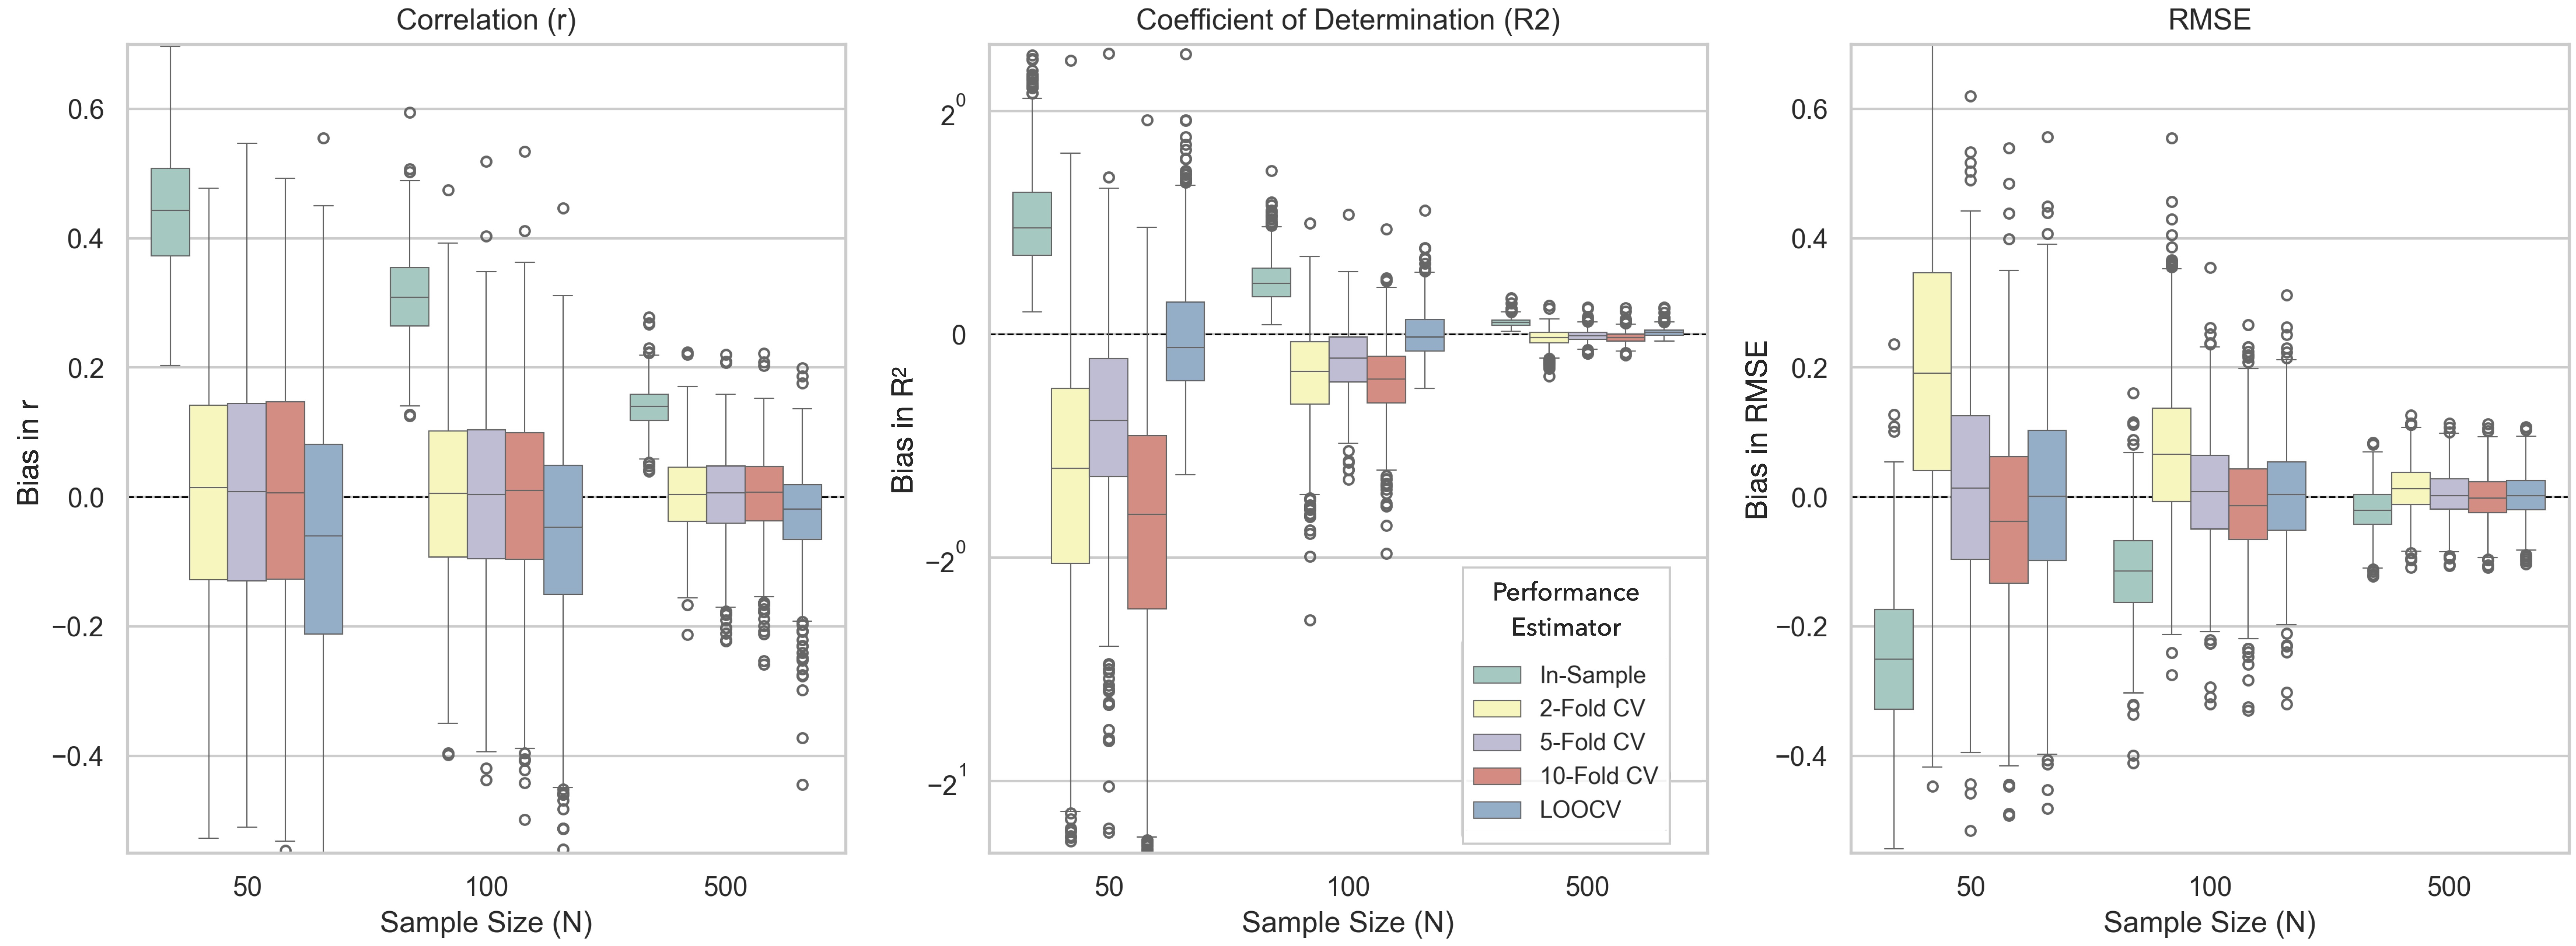
\includegraphics[width=1\textwidth]{fig_s1_bias.jpg}
    \caption{Simulation results of evaluation bias from 1000 sampling iterations. Multiple performance estimators across different sample sizes were color-coded. Three metrics: $r$, $R^2$, and RMSE, were displayed in the column facets.}
    \label{fig:s1_bias}
\end{figure}

The simulation results, depicted in box plots (Figure ~\ref{fig:s1_bias} and ~\ref{fig:s1_var}), explored the evaluation bias and variance distribution. Figure ~\ref{fig:s1_bias} examines the bias alterations across various estimators and sample sizes. Independent of the estimator and metric, the bias diminishes with increasing sample sizes. The in-sample estimator consistently overestimates across all metrics and sample sizes, underscoring the necessity of CV for unbiased performance evaluation. In CV estimators, although LOOCV is traditionally viewed as unbiased, it shows underestimation in model performance, especially when the metric is correlation coefficient (r). Comparatively, 2-, 5-, and 10-fold CV provide a more unbiased estimation than LOOCV for all sample sizes. However, for metrics like $R^2$ or RMSE, LOOCV emerges as the least biased estimator. While K-fold CV exhibits higher bias than LOOCV, this difference dwindles when the sample size exceeds 500. Notably, 10-fold CV, contrary to expectations, demonstrates higher bias than 5-fold CV for small sample sizes (50 and 100) in the $R^2$ metric, though this disparity also becomes insignificant at larger sample sizes.


Considering LOOCV’s singular data point testing, its evaluation variance is pertinent only for RMSE, which permits single data point evaluations. Figure ~\ref{fig:s1_var} illustrates the bias and variance in RMSE across different performance estimators as a function of sample size N. Both bias and variance in RMSE decrease as sample size increases, aligning with the hypothesis. LOOCV provides the least biased estimation, while 2-fold CV exhibits the highest bias without significant reduction at larger sample sizes. However, biases across all estimators converge at a sample size of 500. In terms of evaluation variance, LOOCV consistently shows higher values than other estimators for all sample sizes. Additionally, a lower number of folds K correlates with reduced variance, which is also in line with the hypothesized trend.

\begin{figure}[H]
    \centering
    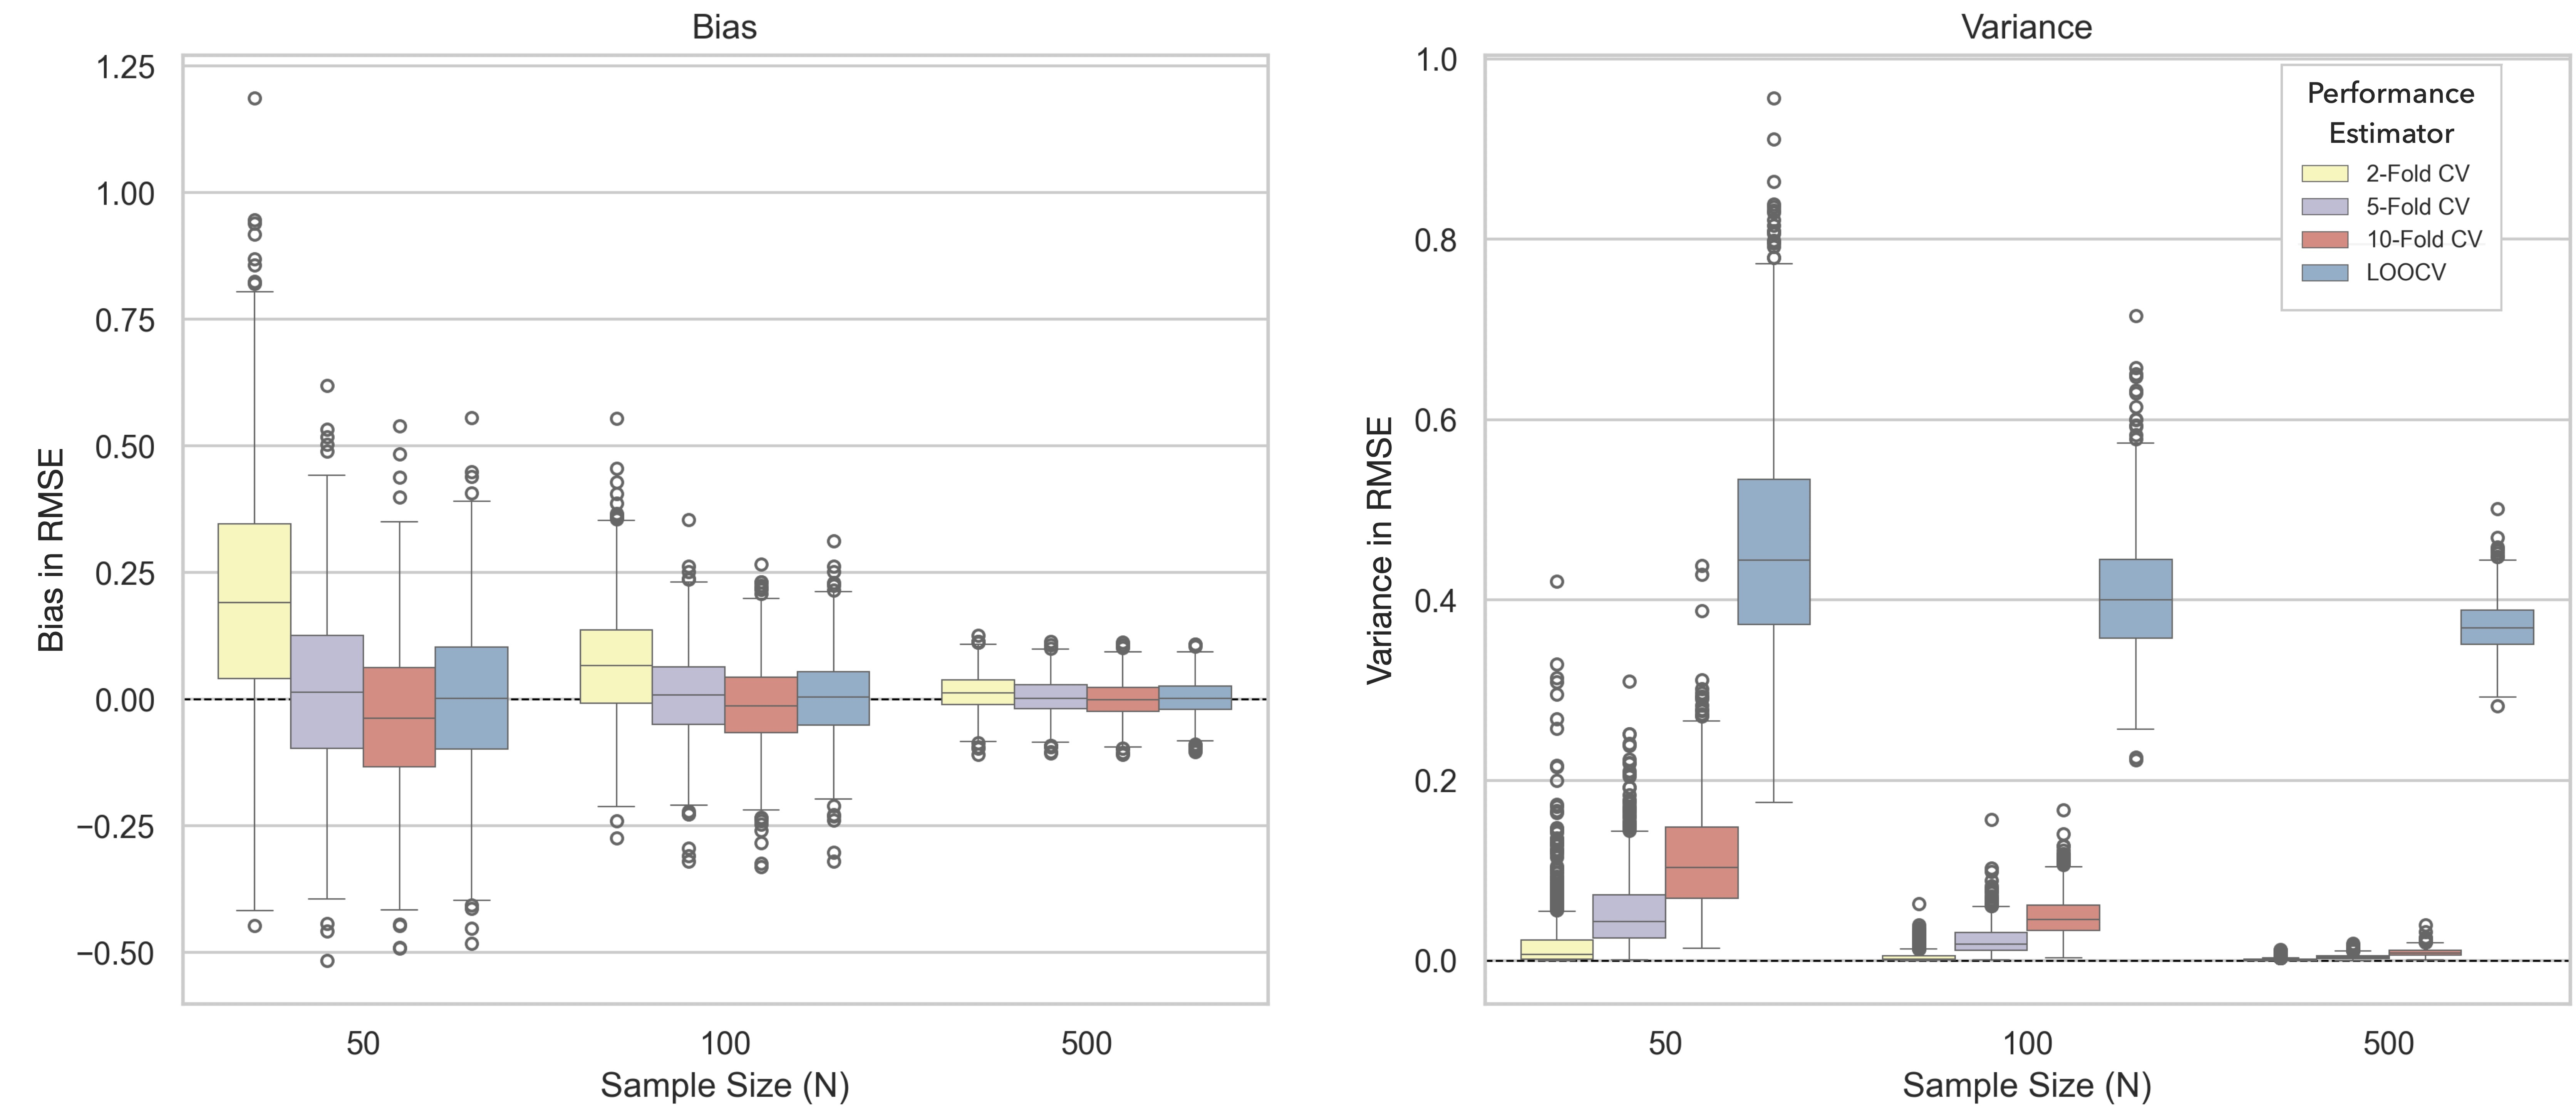
\includegraphics[width=1\textwidth]{fig_s1_var.jpg}
    \caption{Simulation results of evaluation bias and variance from 1000 sampling iterations. Multiple performance estimators across different sample sizes were color-coded. Only RMSE was displayed. Bias and variance were listed in the left and right facets, respectively.}
    \label{fig:s1_var}
\end{figure}

In conclusion, when conducting model evaluation, it is crucial to consider the estimator and sample size, as they significantly influence evaluation reliability which can be decomposed into bias and variance. Larger sample sizes generally lead to reduced bias and variance, enhancing the reliability of the evaluation process. For unbiased performance estimation, CV methods, such as K-fold CV and LOOCV, are preferable to in-sample estimation. LOOCV often provides less biased estimations for certain metrics but can exhibit higher variance. It is also noteworthy that the number of folds in K-fold CV can affect bias and variance; thus, experimenting with different numbers of folds, especially in smaller sample sizes, can be beneficial. Ultimately, the selection of appropriate evaluation techniques should be tailored to the specific context of the dataset and the objectives of the modeling exercise, ensuring a robust and reliable assessment of model performance.

\subsection{Study 2: Misuse of Model Selection Can Lead to Over-Optimistic Performance Estimates}

The evaluation bias was visualized using box plots (Figure ~\ref{fig:s2_results}), with the feature selection factor (FS) on the x-axis and hyperparameter tuning (HT) distinguished by color — green for incorrect and yellow for correct implementation. The y-axis represents the evaluation bias as measured by the correlation coefficient. The results indicate a clear overestimation of model performance when feature selection is applied to the entire dataset, regardless of hyperparameter tuning. The median biases were 0.797 for “FS=0; HT=0” and 0.761 for “FS=0; HT=1”. Moreover, inappropriate evaluation in hyperparameter tuning resulted in a significant bias (p-value < 0.001) with a median of 0.113 for “FS=1; HT=0”. The only scenario without bias significantly occurred when both feature selection and hyperparameter tuning were correctly incorporated within the cross-validation process “FS=1; HT=1”, yielding a median bias of -0.008. These findings align with the initial hypothesis and the prevailing literature, reinforcing that model selection must be integrated into the cross-validation workflow to prevent an overestimation of model performance.

\begin{figure}
    \centering
    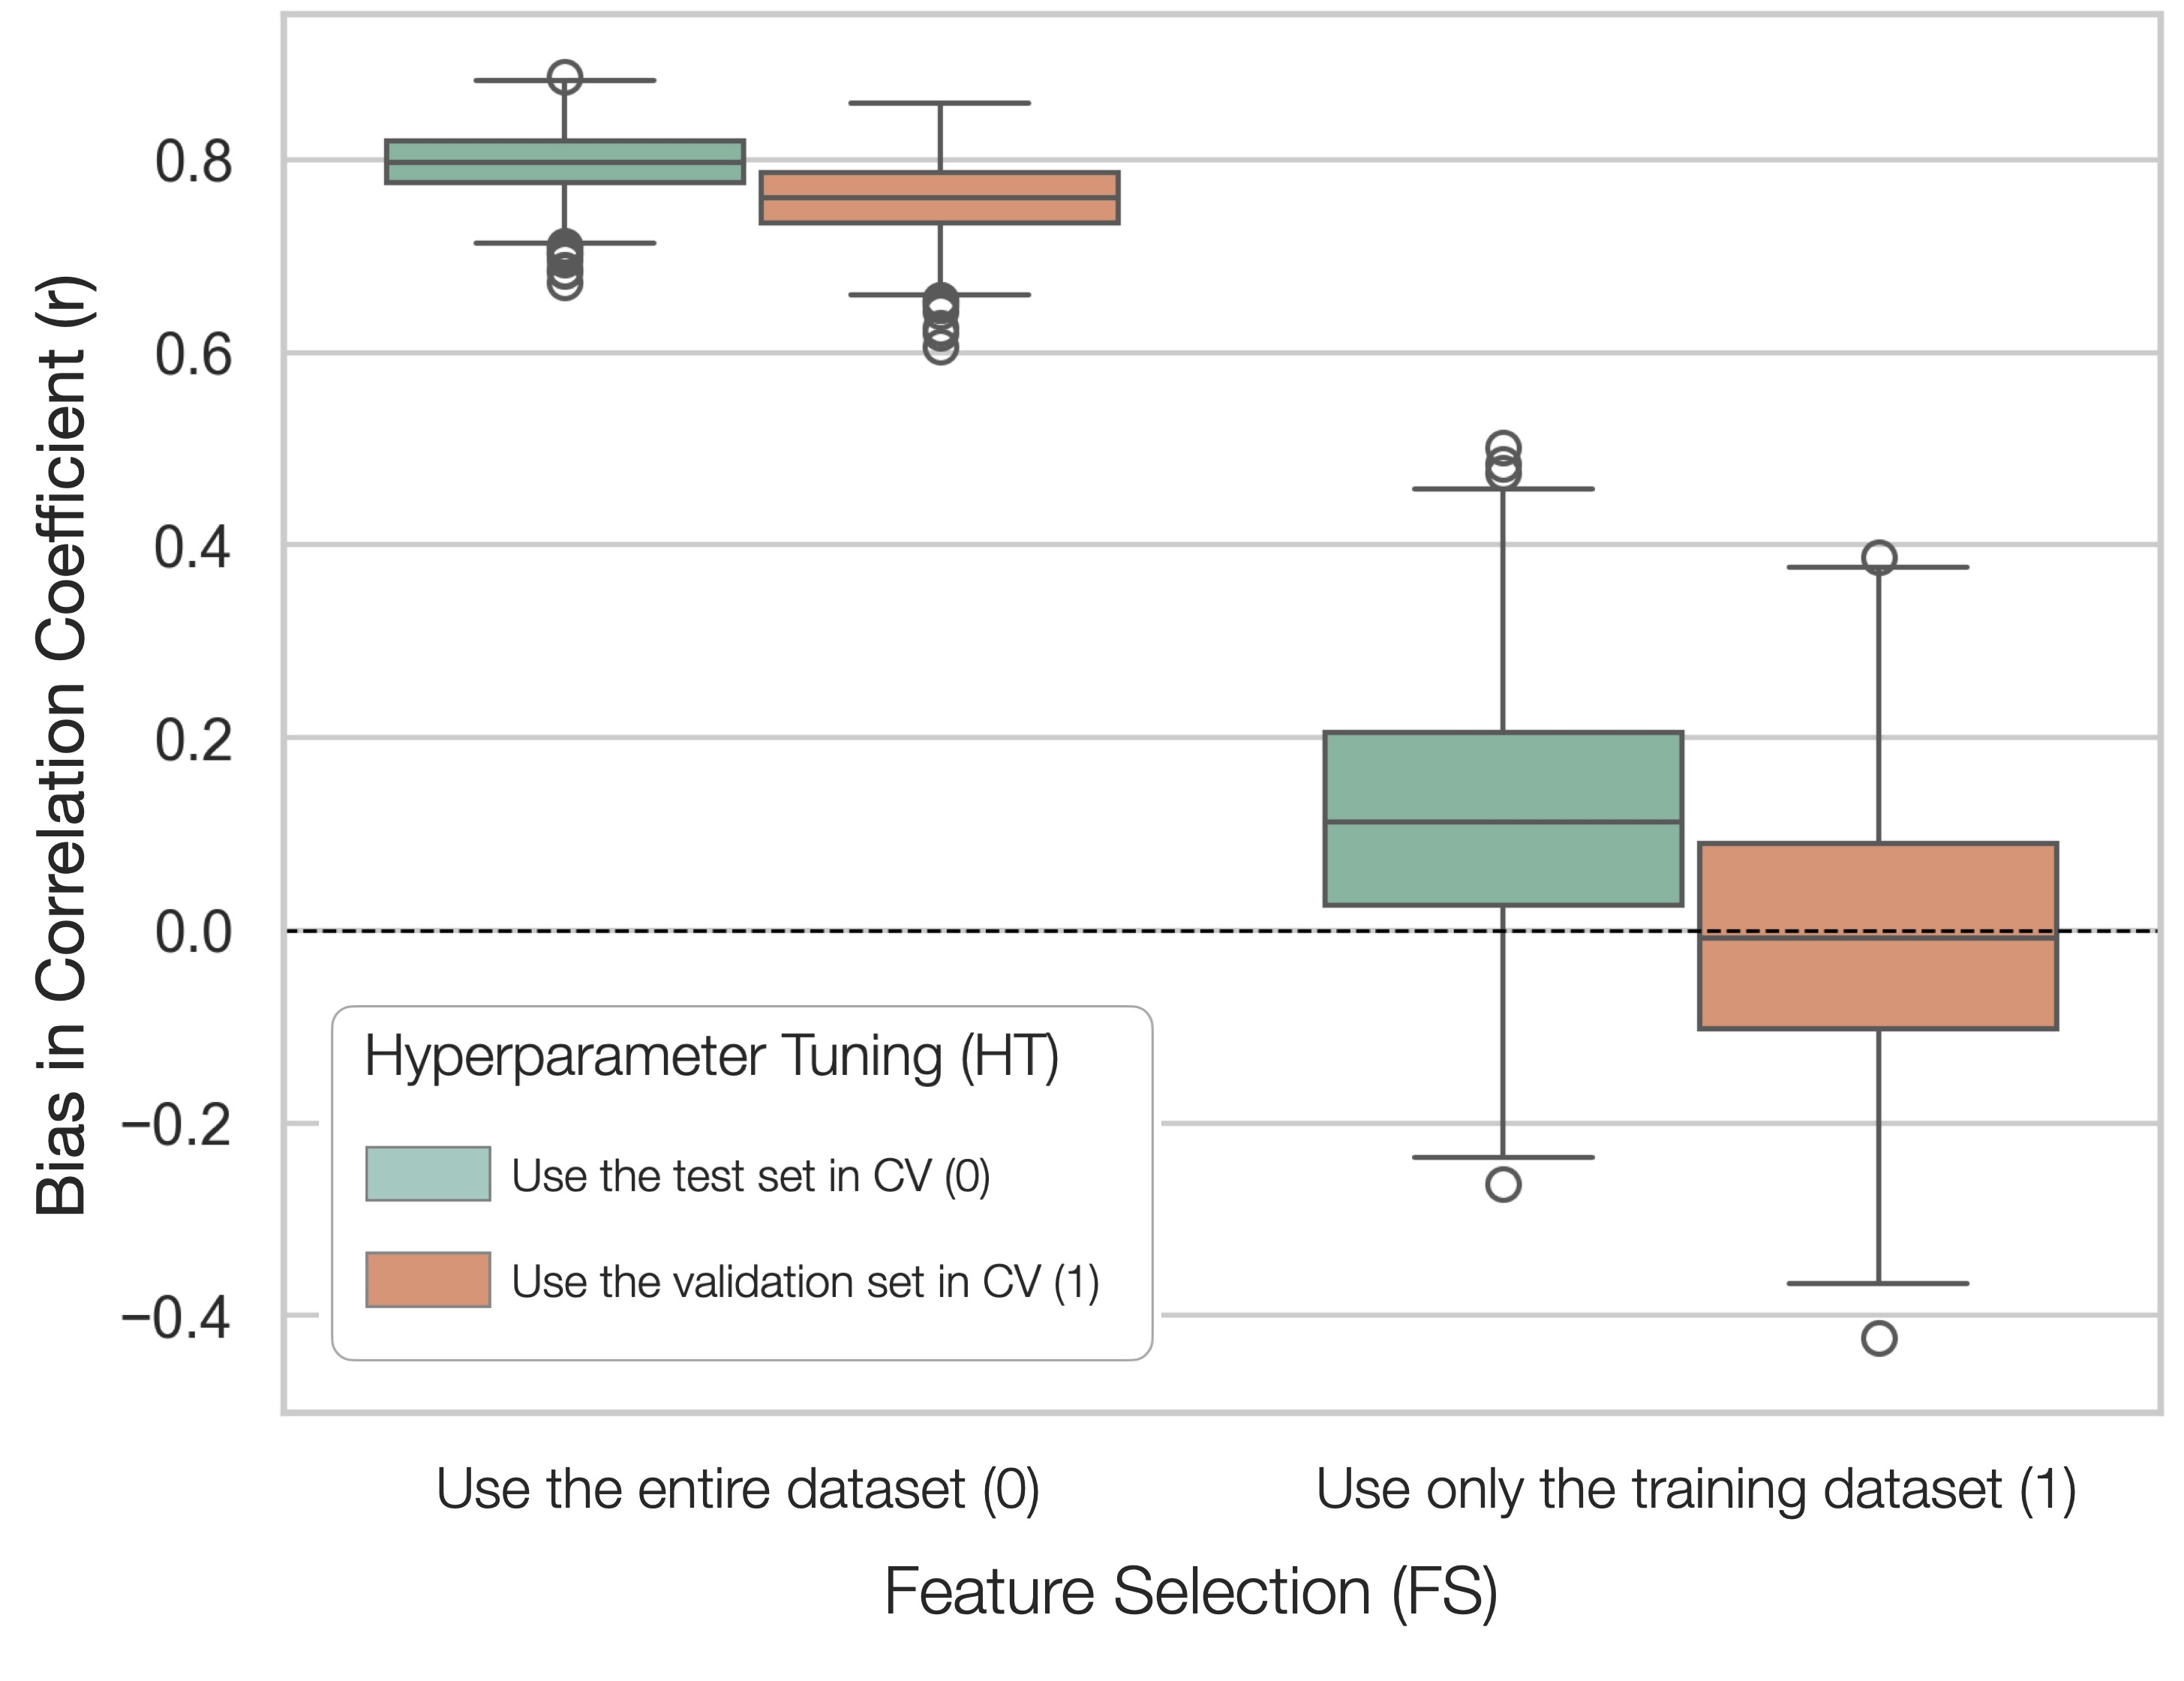
\includegraphics[width=.7\textwidth]{fig_s2_results.jpg}
    \caption{The evaluation bias of the four model selection strategies.}
    \label{fig:s2_results}
\end{figure}

The simulation results robustly confirm the hypothesis that improper implementation of model selection inflates performance estimates. Specifically, the evaluation bias is markedly high when feature selection precedes data splitting, with or without correct hyperparameter tuning. Although integrating feature selection within cross-validation folds mitigates this bias, incorrect hyperparameter tuning still significantly skews performance metrics. Notably, this overestimation from the hyperparameter tuning is even more pronounced in complex models, such as neural network architectures that often entail over a million parameters. These findings underscore the necessity of meticulous cross-validation practices, particularly for feature selection and hyperparameter tuning, to ensure accurate performance estimations and generalizability in predictive modeling.

\subsection{Study 3: Overlooking Experimental Block Effects Can Lead to Biased Model Performance Estimates}

In this simulation, an ANOVA table (Table ~\ref{tab:anova}), calculated from a single iteration for illustrative purposes, demonstrates that the simulated data exhibits block variation significantly greater than the residual variance. The result (Figure ~\ref{fig:s3_results}) shows that regardless of the amplitude of block effects in this simulation study, the Block CV strategy consistently yields a mean performance estimate close to zero, while the Random CV strategy consistently and significantly overestimates the model performance (p-value < 0.001). This finding supports the hypothesis that Random CV tends to overestimate model performance when block variation predominates over residual variation.

\begin{table}
    \caption{ANOVA results for a single iteration of the simulated data with b = 0.5. SS: sum of squares; DF: degree of freedom; MS: mean square; F: F-statistic}
    \centering
    \begin{tabular}{lccccc}
        \toprule
        Source & SS & DF & MS & F & p-value \\
        \midrule
        Between & 60.971 & 4 & 15.243 & 20.580 & <0.001 \\
        Within & 70.363 & 95 & 0.741 & &  \\
        \cmidrule(r){1-3}
        Total & 131.35 & 99 & & & \\
        \bottomrule
    \end{tabular}
    \label{tab:anova}
\end{table}

In conclusion, block CV proves to be a vital tool in assessing the generalizability and accuracy of a predictive model, especially in contexts where block effects, such as herd variations, play a significant role in both the predicting features and response variable. The random CV strategy, which randomly assigns samples to folds without considering block effects, tends to overestimate model performance. This study recommends that block CV be used as a benchmark in model evaluation, especially when block effects are present

\begin{figure}
    \centering
    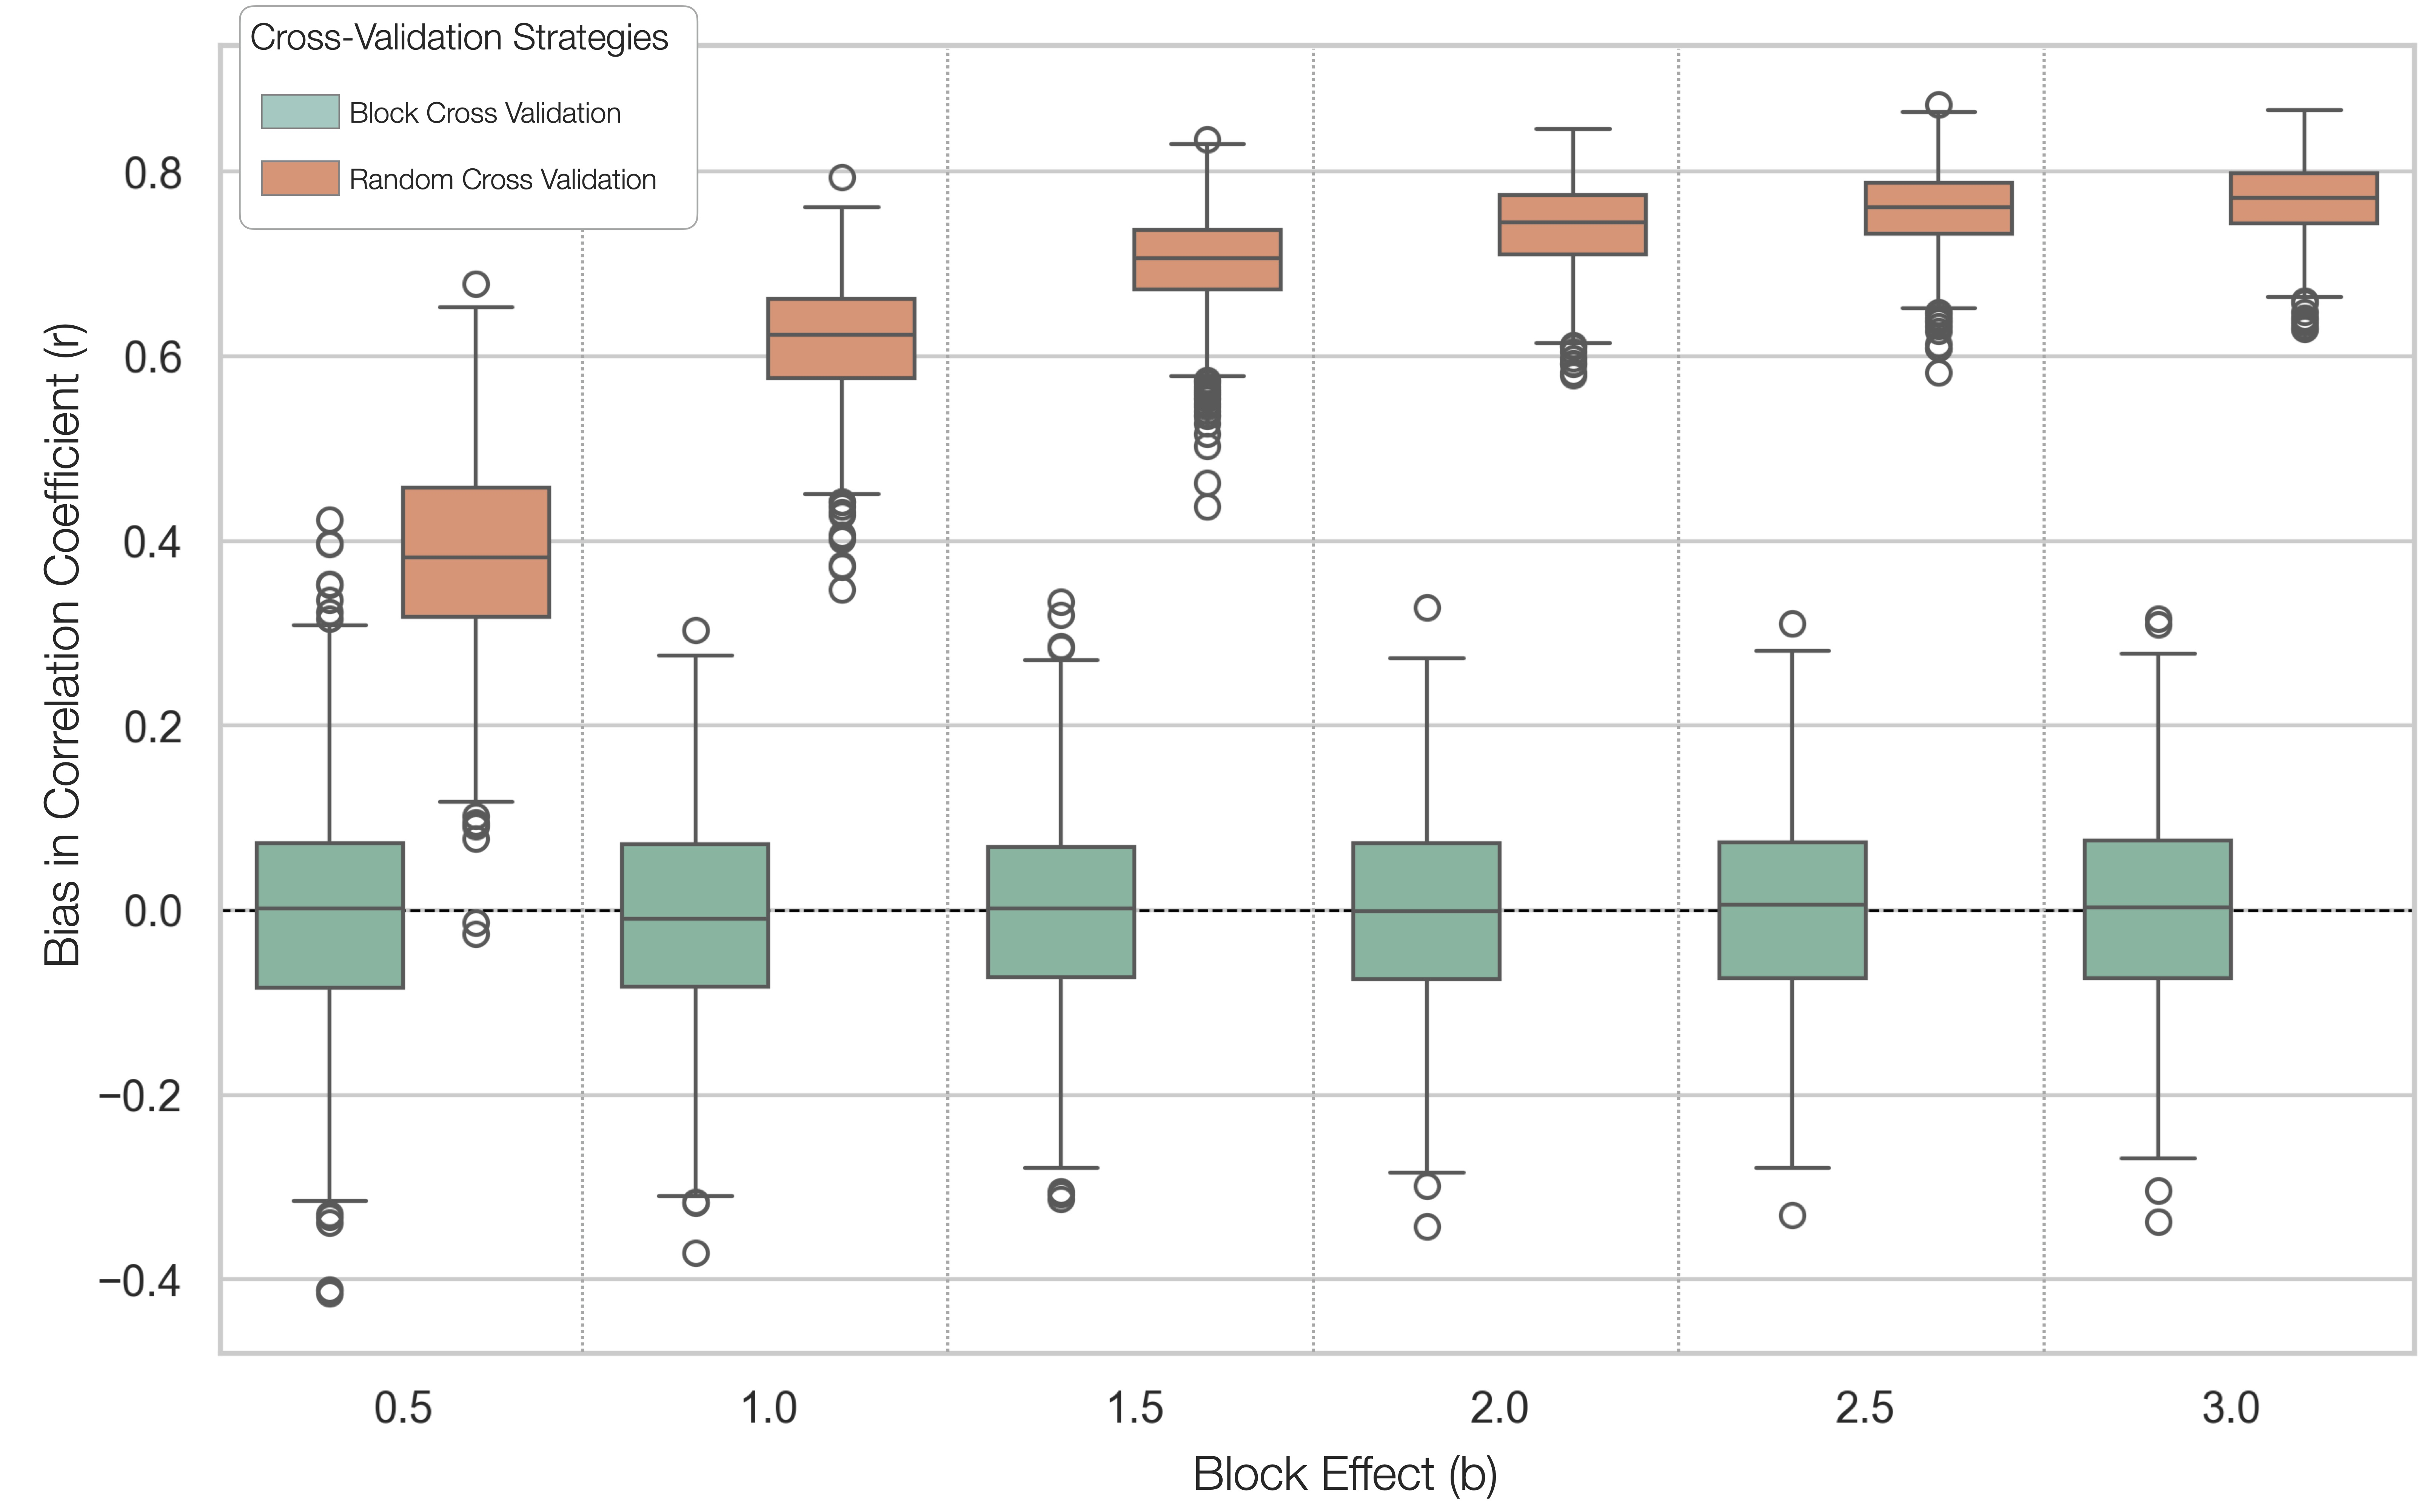
\includegraphics[width=1\textwidth]{fig_s3_results.jpg}
    \caption{Bias in model performance estimation by Block CV and Random CV across 1000 iterations. The dashed line represents the null hypothesis that the mean performance estimate is zero.}
    \label{fig:s3_results}
\end{figure}

\subsection{Study 4: Different Regression Metrics Illustrate Different Aspects of Model Performance}

\begin{figure}
    \centering
    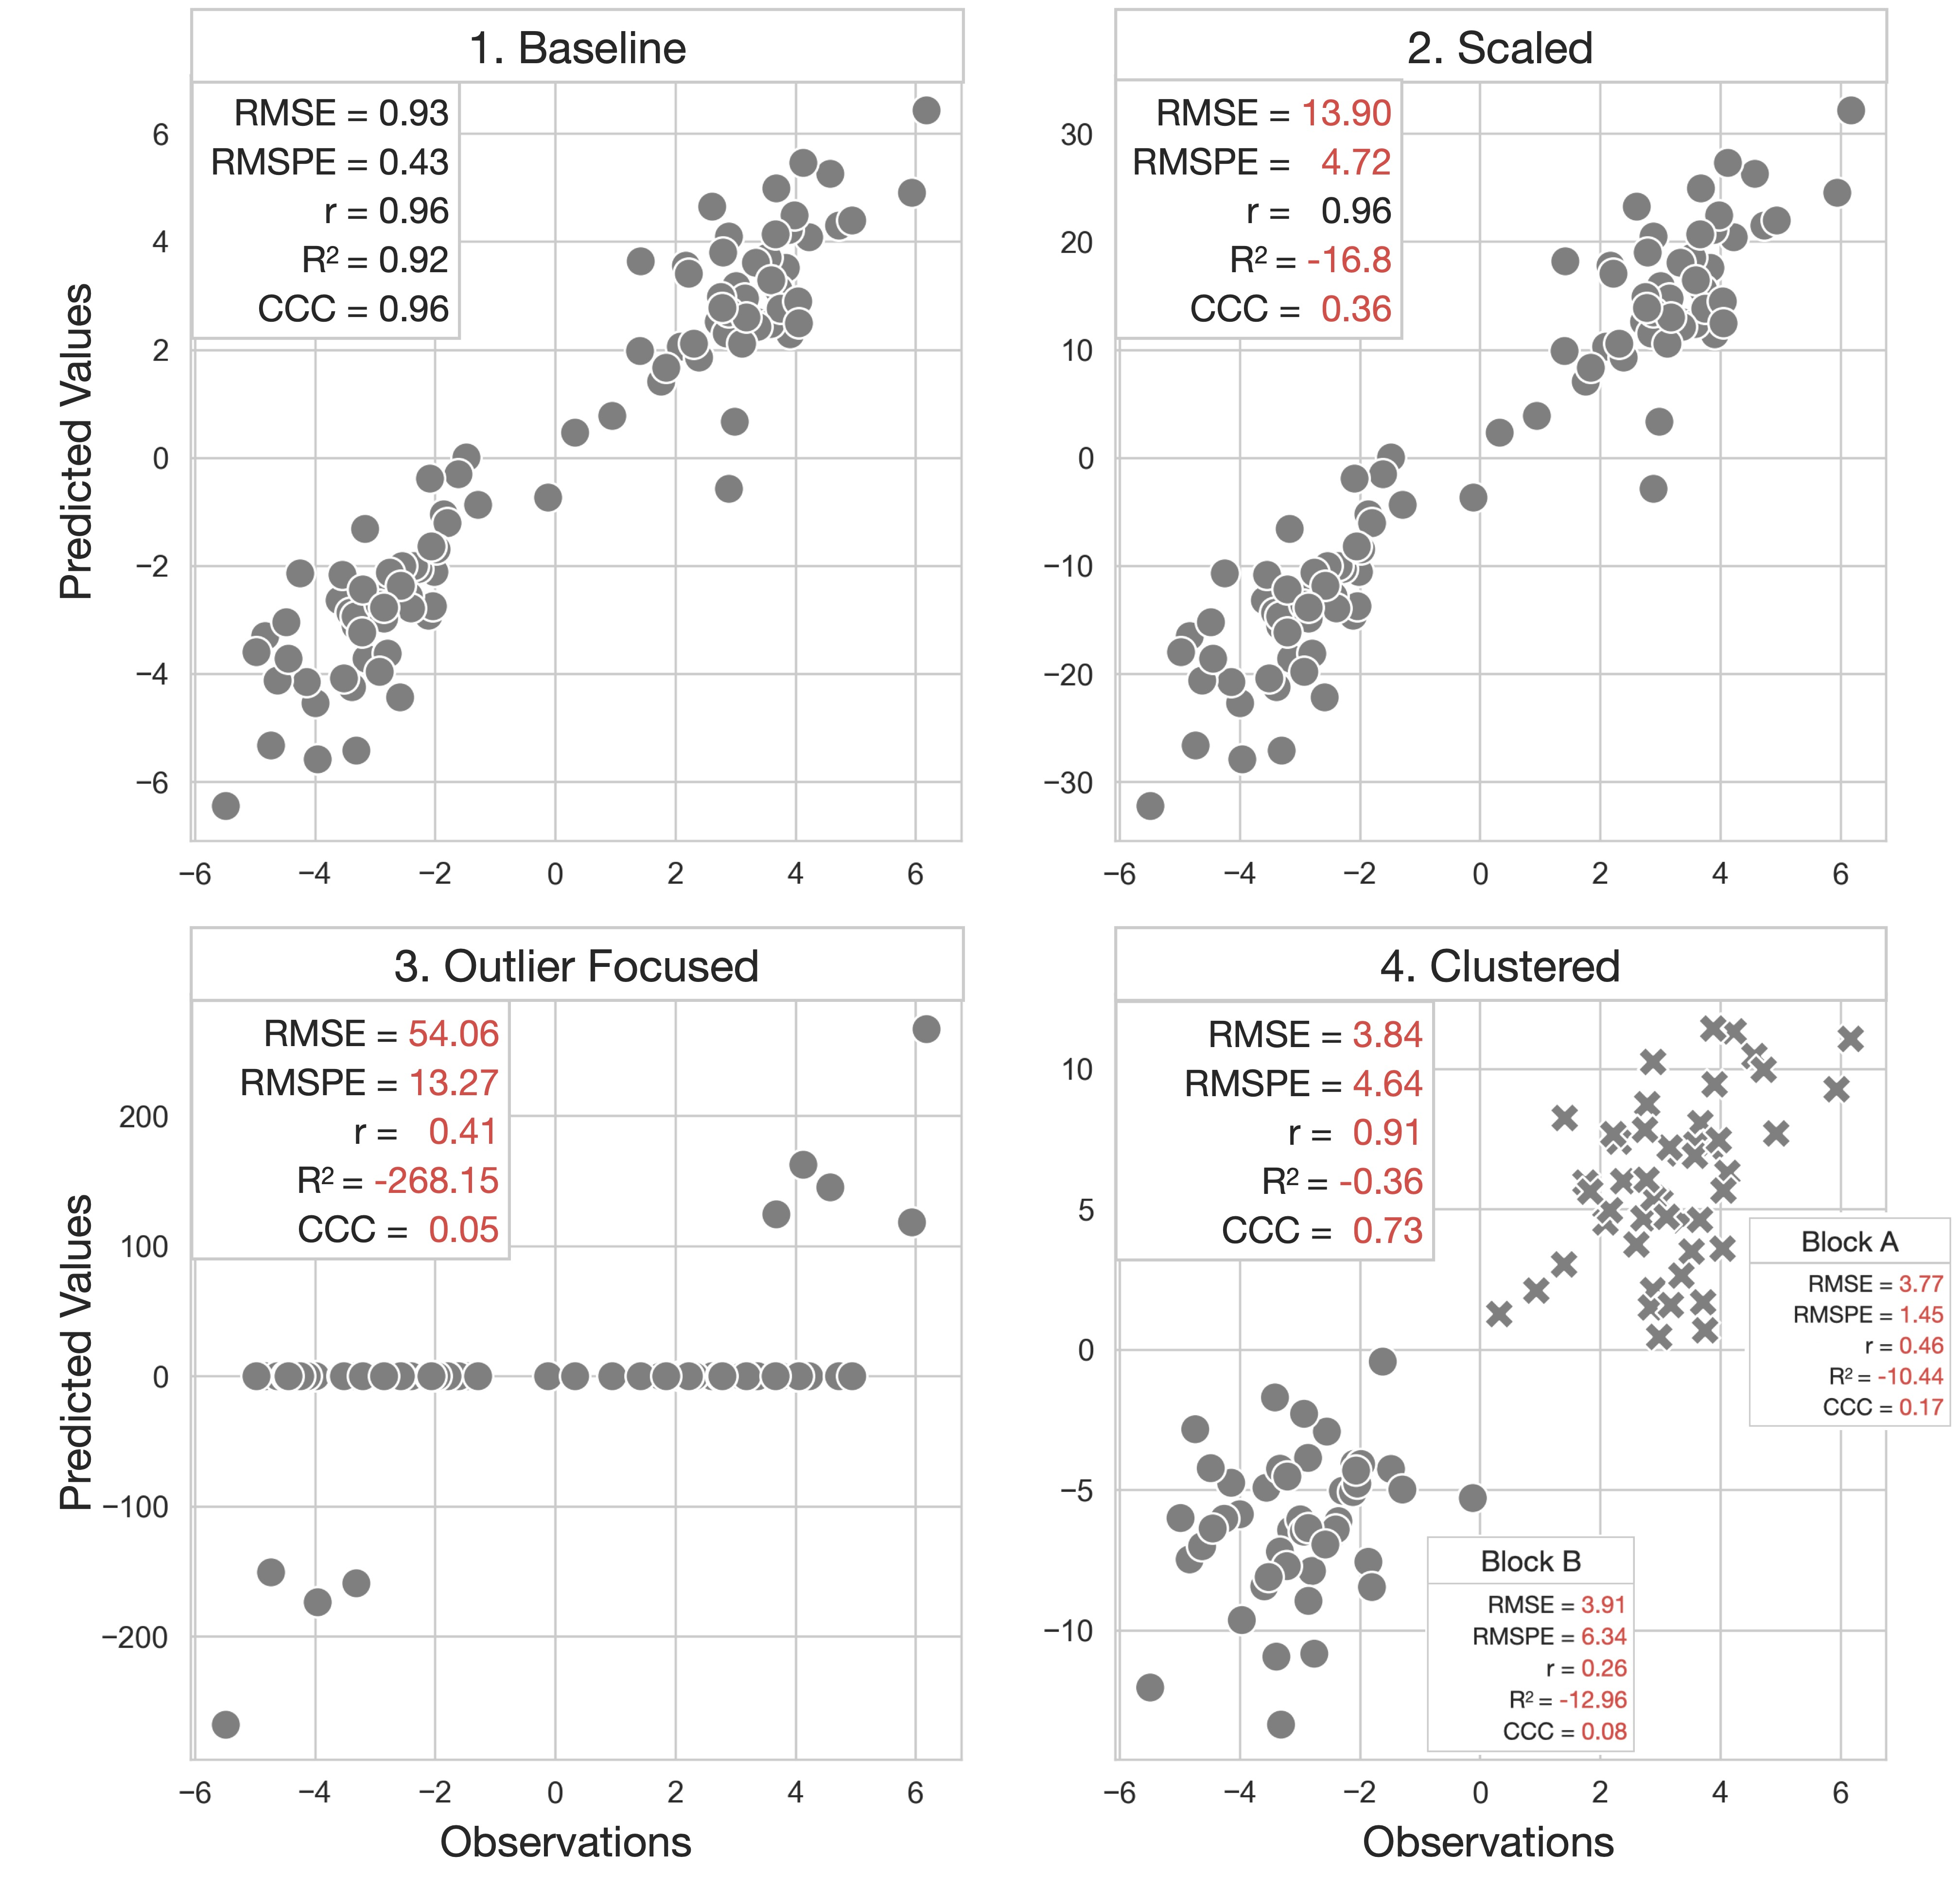
\includegraphics[width=.9\textwidth]{fig_s4_reg.jpg}
    \caption{Scatter plots display the same observations against four different prediction scenarios in the given hypothetical example. Scenario "Baseline" serves as a baseline for the metrics, with any metric better than the baseline highlighted in bold and underscored, and any worse metric colored in red.}
    \label{fig:s4_reg}
\end{figure}

The simulated hypothetical example in Figure ~\ref{fig:s4_reg} illustrates the performance of four different prediction scenarios. The error-based metrics, RMSE and RMSPE, are sensitive to the magnitude of the error. In Scenario "Scaled", where the errors are five times larger but remain the same in rank order compared to Scenario "Baseline", the RMSE inflates from 0.93 to 13.90, and RMSPE also increases from 0.43 to 4.72. Another notable characteristic of RMSE and RMSPE is that they weigh more on large errors, which is essential when making a large error is costly and should be prioritized for avoidance. In Scenario "Outliers", where certain predictions deviate substantially from the majority, the squaring operation in Equation ~\ref{eq_rmse} accentuates these outliers, culminating in an RMSE of 54.06 and RMSPE of 13.27. However, when investigating into the intra-block performance in the scenario "Clustered", the RMSE failed to detect the inflated performance due to the strong block effects. It resulted in a similar RMSE of 3.84 from the entire prediction set and 3.77 and 3.91 within each block. This phenomenon emphasizes again that RMSE is affected solely by the magnitude of the error, which neglects the ability of the model to capture relative trends in intra-block or inter-block predictions.
On the other hand, when the goal is to rank observations of interest rather than predict the absolute magnitude of the error, linearity-based metrics can provide more insights. The correlation $r$ is an example showing its consistency across the Scenario "Baseline" and "Scaled", despite the latter having five times larger errors. This metric is particularly useful when the relative order of predictions is more important than the absolute error magnitude. However, it is worth noting that the correlation $r$ can be misleading in certain scenarios, such as the Scenario "Outlier Focused", where 90\% of the predictions are zero. In this case, the correlation $r$ show a moderate performance of 0.41, which is mainly contributed by the 10\% of the outlier predictions that are "ranked" correctly but with a large error magnitude. This example highlights the importance of visually inspecting the regression results through scatter plots to avoid misleading conclusions. Moreover, one common pitfall of the correlation $r$ is that block effects can influence it, leading to an inflated performance estimate if individual variation is of greater interest than inter-block variation. This was demonstrated in Scenario "Clustered", where the overall coefficient $r$ was 0.91, but the metric within each block was only 0.46 and 0.26, respectively. Therefore, it is essential to examine regression results within identifiable blocks. Besides the correlation $r$, $R^2$ provides a more comprehensive insight, as it focuses both the linear trend from the variance composition and the error magnitude from the residual sum of squares. From the "Scaled" scenario, $R^2$ successfully detected the inflated error magnitude, resulting in a negative value of -16.8. It also captured the outlier-induced variance in the "Outliers" scenario, with a negative value of -268.15. Lastly, in Scenario "Clustered", the value of $R^2$ indicated a weak performance by the model with a score of -0.36. This score is statistically reasonable, as the predictions have larger variance than the observations. The metric also successfully detected the model failure in capturing intra-block variation, as the $R^2$ values within each block were -10.44 and -12.96, respectively. However, an obvious limitation of $R^2$ is that it has no standard scale. Considering this, a more nuanced evaluation metric, $CCC$, showcases a more balanced performance evaluation. It always range from -1 to 1, and it successfully captures all the characteristics of the four scenarios. In Scenario "Scaled", the $CCC$ value dropped from 0.96 to 0.36. In Scenario "Outliers", the $CCC$ value plummeted to 0.05, showcasing the model's failure to "align" the predictions with the observations with 90\% of the predictions being zero. In the Scenario "Clustered", although the $CCC$ value was 0.73, the metric also showed the model's weakness in each block, with the $CCC$ values of 0.17 and 0.08, respectively. This study demonstrates that $CCC$ is a more balanced metric that considers both the linear trend and the error magnitude, making it a more comprehensive evaluation metric for regression models.

\subsection{Study 5: Label-Invariant Metrics Provide Balanced Assessment in Binary Classification}

\begin{figure}[h]
    \centering
    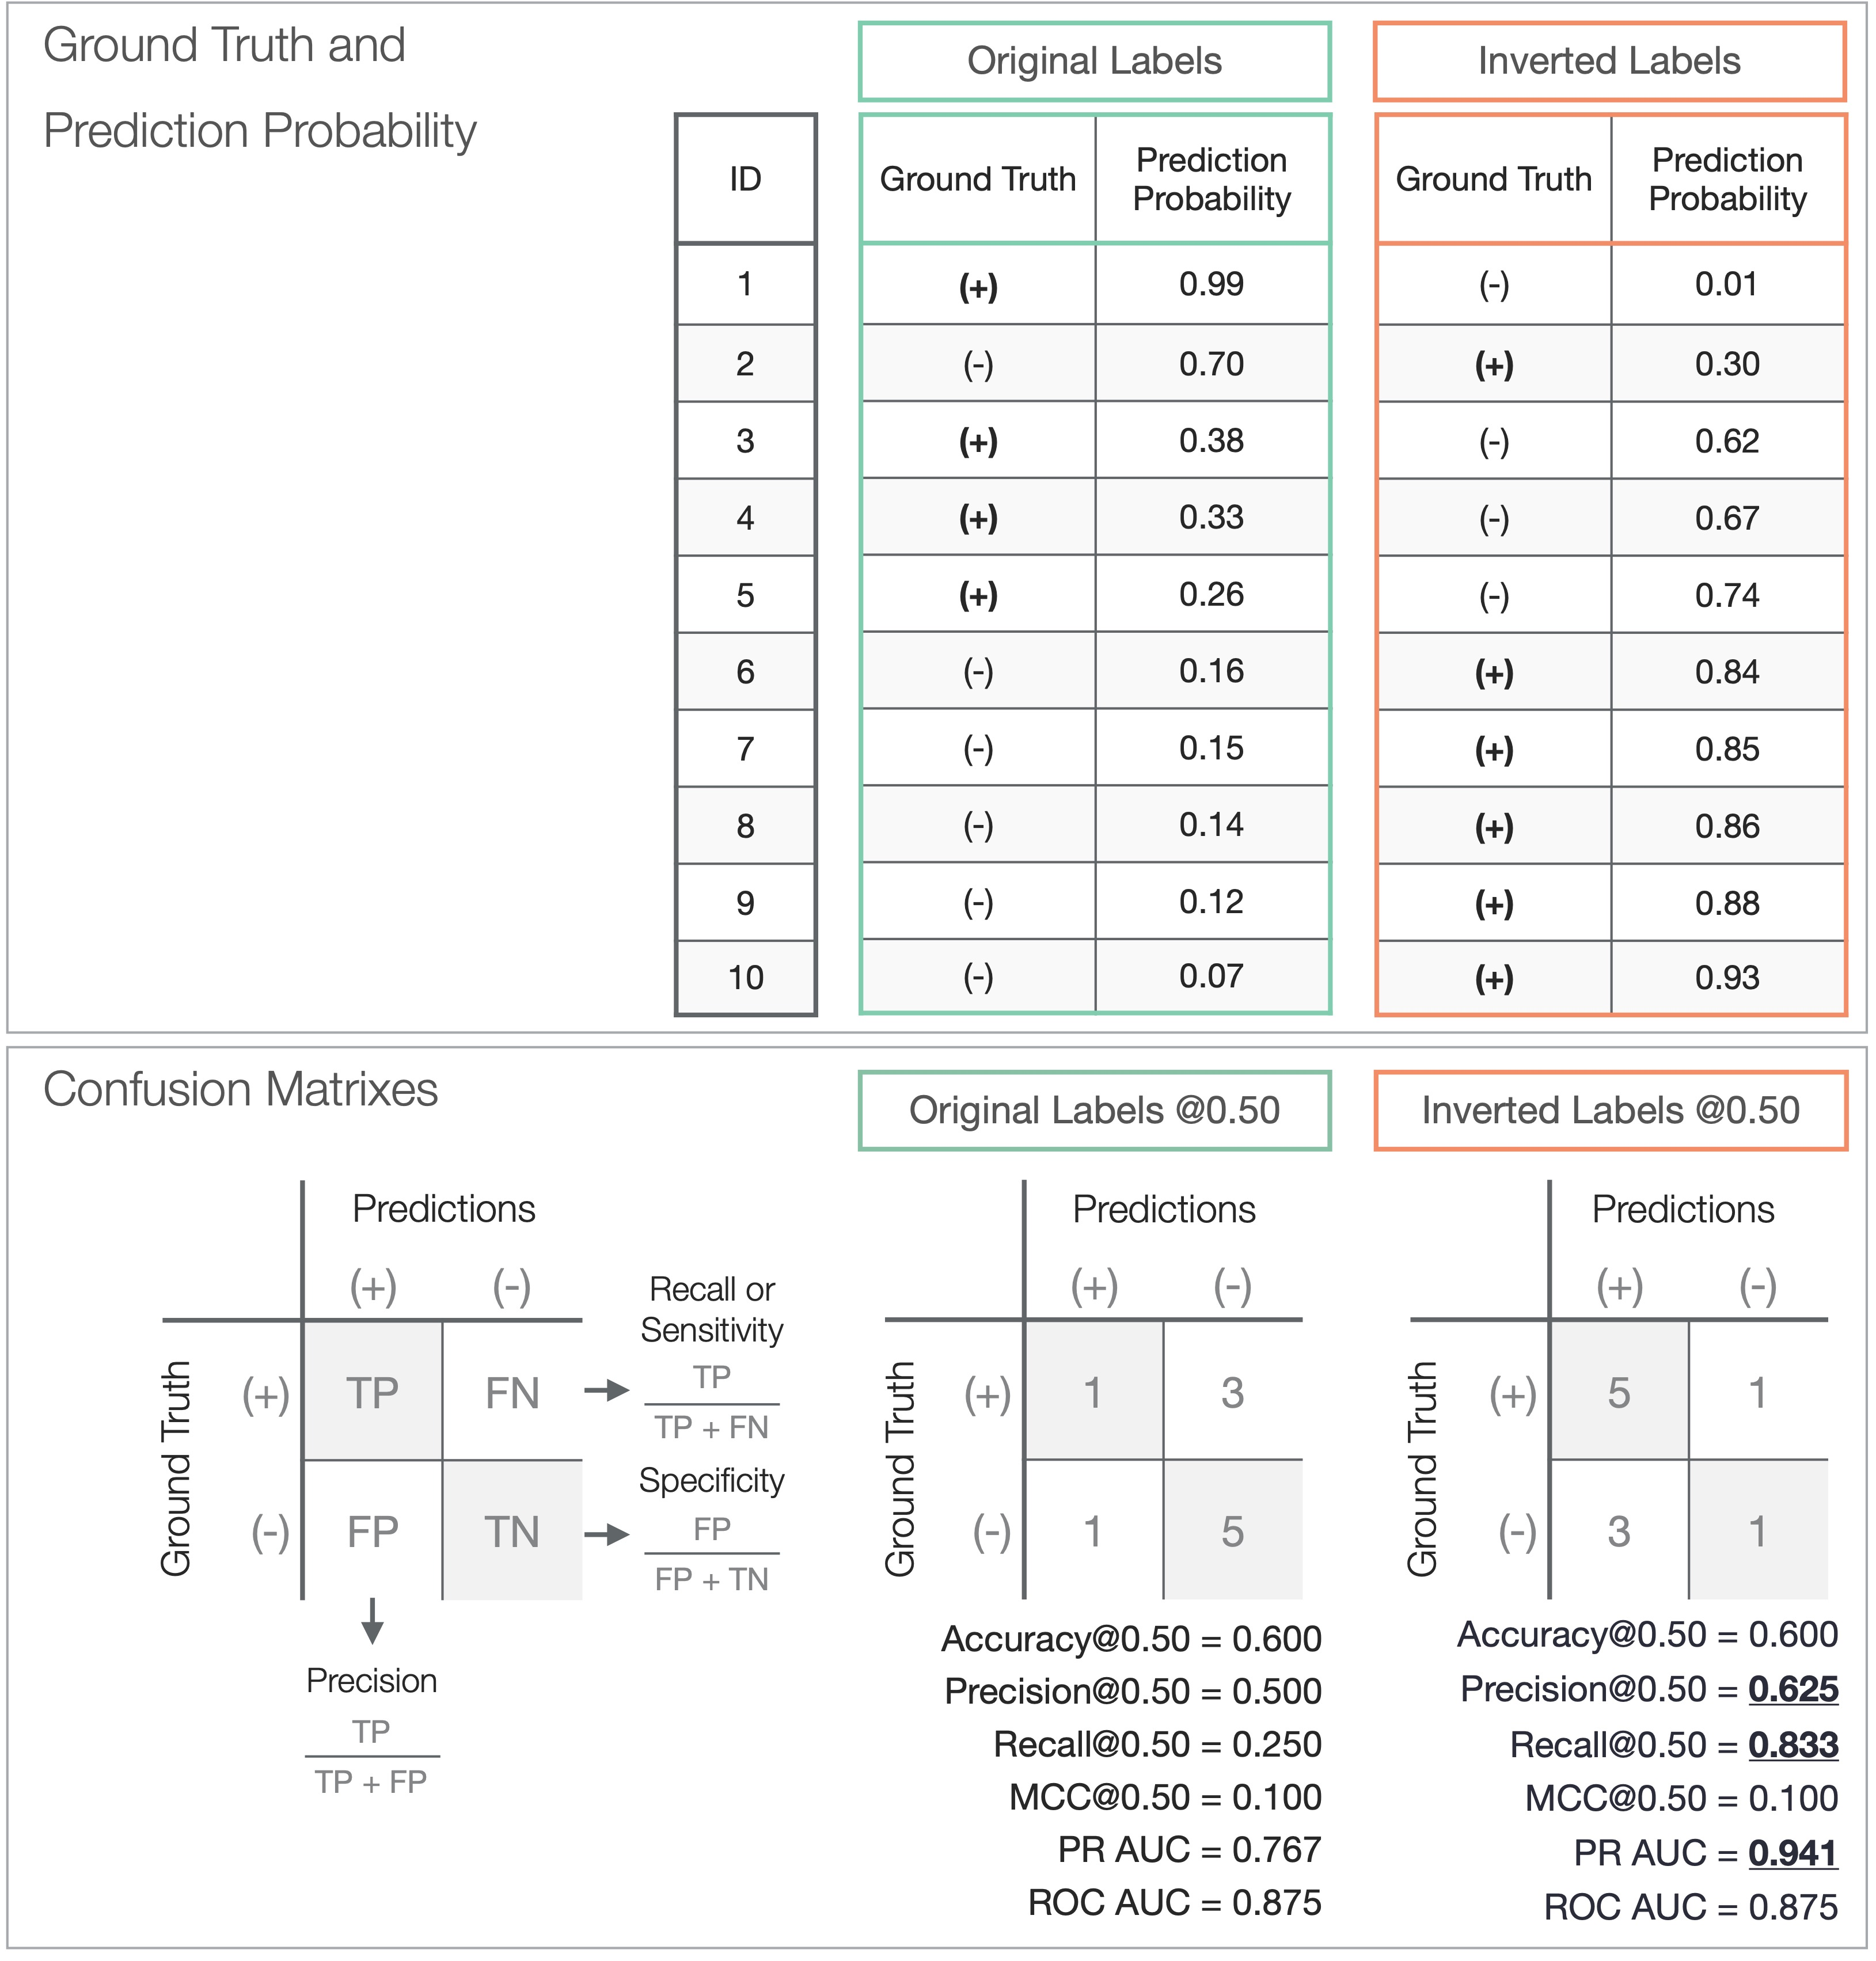
\includegraphics[width=.8\textwidth]{fig_s5_cls.jpg}
    \caption{Simulated hypothetical example of binary classification. TP: true positive; FN: false negative; FP: false positive; TN: true negative; \textbf{Upper}: The ground truth and prediction probability. \textbf{Lower}: The confusion matrix of the prediction at a threshold of 0.5, followed by classification metrics of accuracy, precision, recall, MCC, PR curve AUC, and ROC curve AUC. The performance of the original labels serves as a baseline for comparison. Any better performance metrics from the inverted labels are highlighted in bold and underscored}
    \label{fig:s5_cls}
\end{figure}


Different metrics in binary classification were evaluated in a simulated example (Figure ~\ref{fig:s5_cls}). The original labels were inverted to examine the robustness of the metrics against label choices. The accuracy metric, with a 0.5 threshold in this example, stands at 0.60. This figure might suggest modest efficacy, marginally surpassing random chance, with an accuracy of 0.50. Nonetheless, the same accuracy level could be achieved by classifying every sample as negative in an imbalanced dataset where negatives are predominant. In contrast, precision and recall provide a more nuanced evaluation of model performance by separately assessing the correctness of positive predictions and the ability to detect actual positives. With a threshold of 0.5, the example dataset yields precision and recall values of 0.5 and 0.25, respectively. These metrics deliver more interpretable information that only half of the positive predictions are correct, and just a quarter of the actual positives are detected. This contrasts with an accuracy of 0.6, which may appear misleadingly high due to the abundance of negative samples.
Additionally, it is noted that the chosen confidence threshold significantly impacts precision and recall. While the trade-off between these two metrics is not always linear, it is generally observed that a higher threshold increases precision but decreases recall, and vice versa. A high threshold indicates a conservative approach in predicting positives, reducing false positives, and thus enhancing precision. However, this often leads to missing actual positive cases, lowering recall. Hence, the Precision-Recall (PR) curve is an essential tool for evaluating model performance across various thresholds. Plotted with recall on the x-axis and precision on the y-axis, this curve is derived by computing these metrics at different thresholds (Figure ~\ref{fig:s5_curve}, Left). The Area Under the Curve (AUC) provides a summary measure of the PR curve's overall performance. A model's effectiveness is generally indicated by how close a point on the PR curve is to the top-right corner. For example, at a threshold of 0.25, which is positioned near the top-right of the PR curve, the model demonstrates impressive performance with an accuracy of 0.90, precision of 0.80, and recall at 1.00.

\begin{figure}[h]
    \centering
    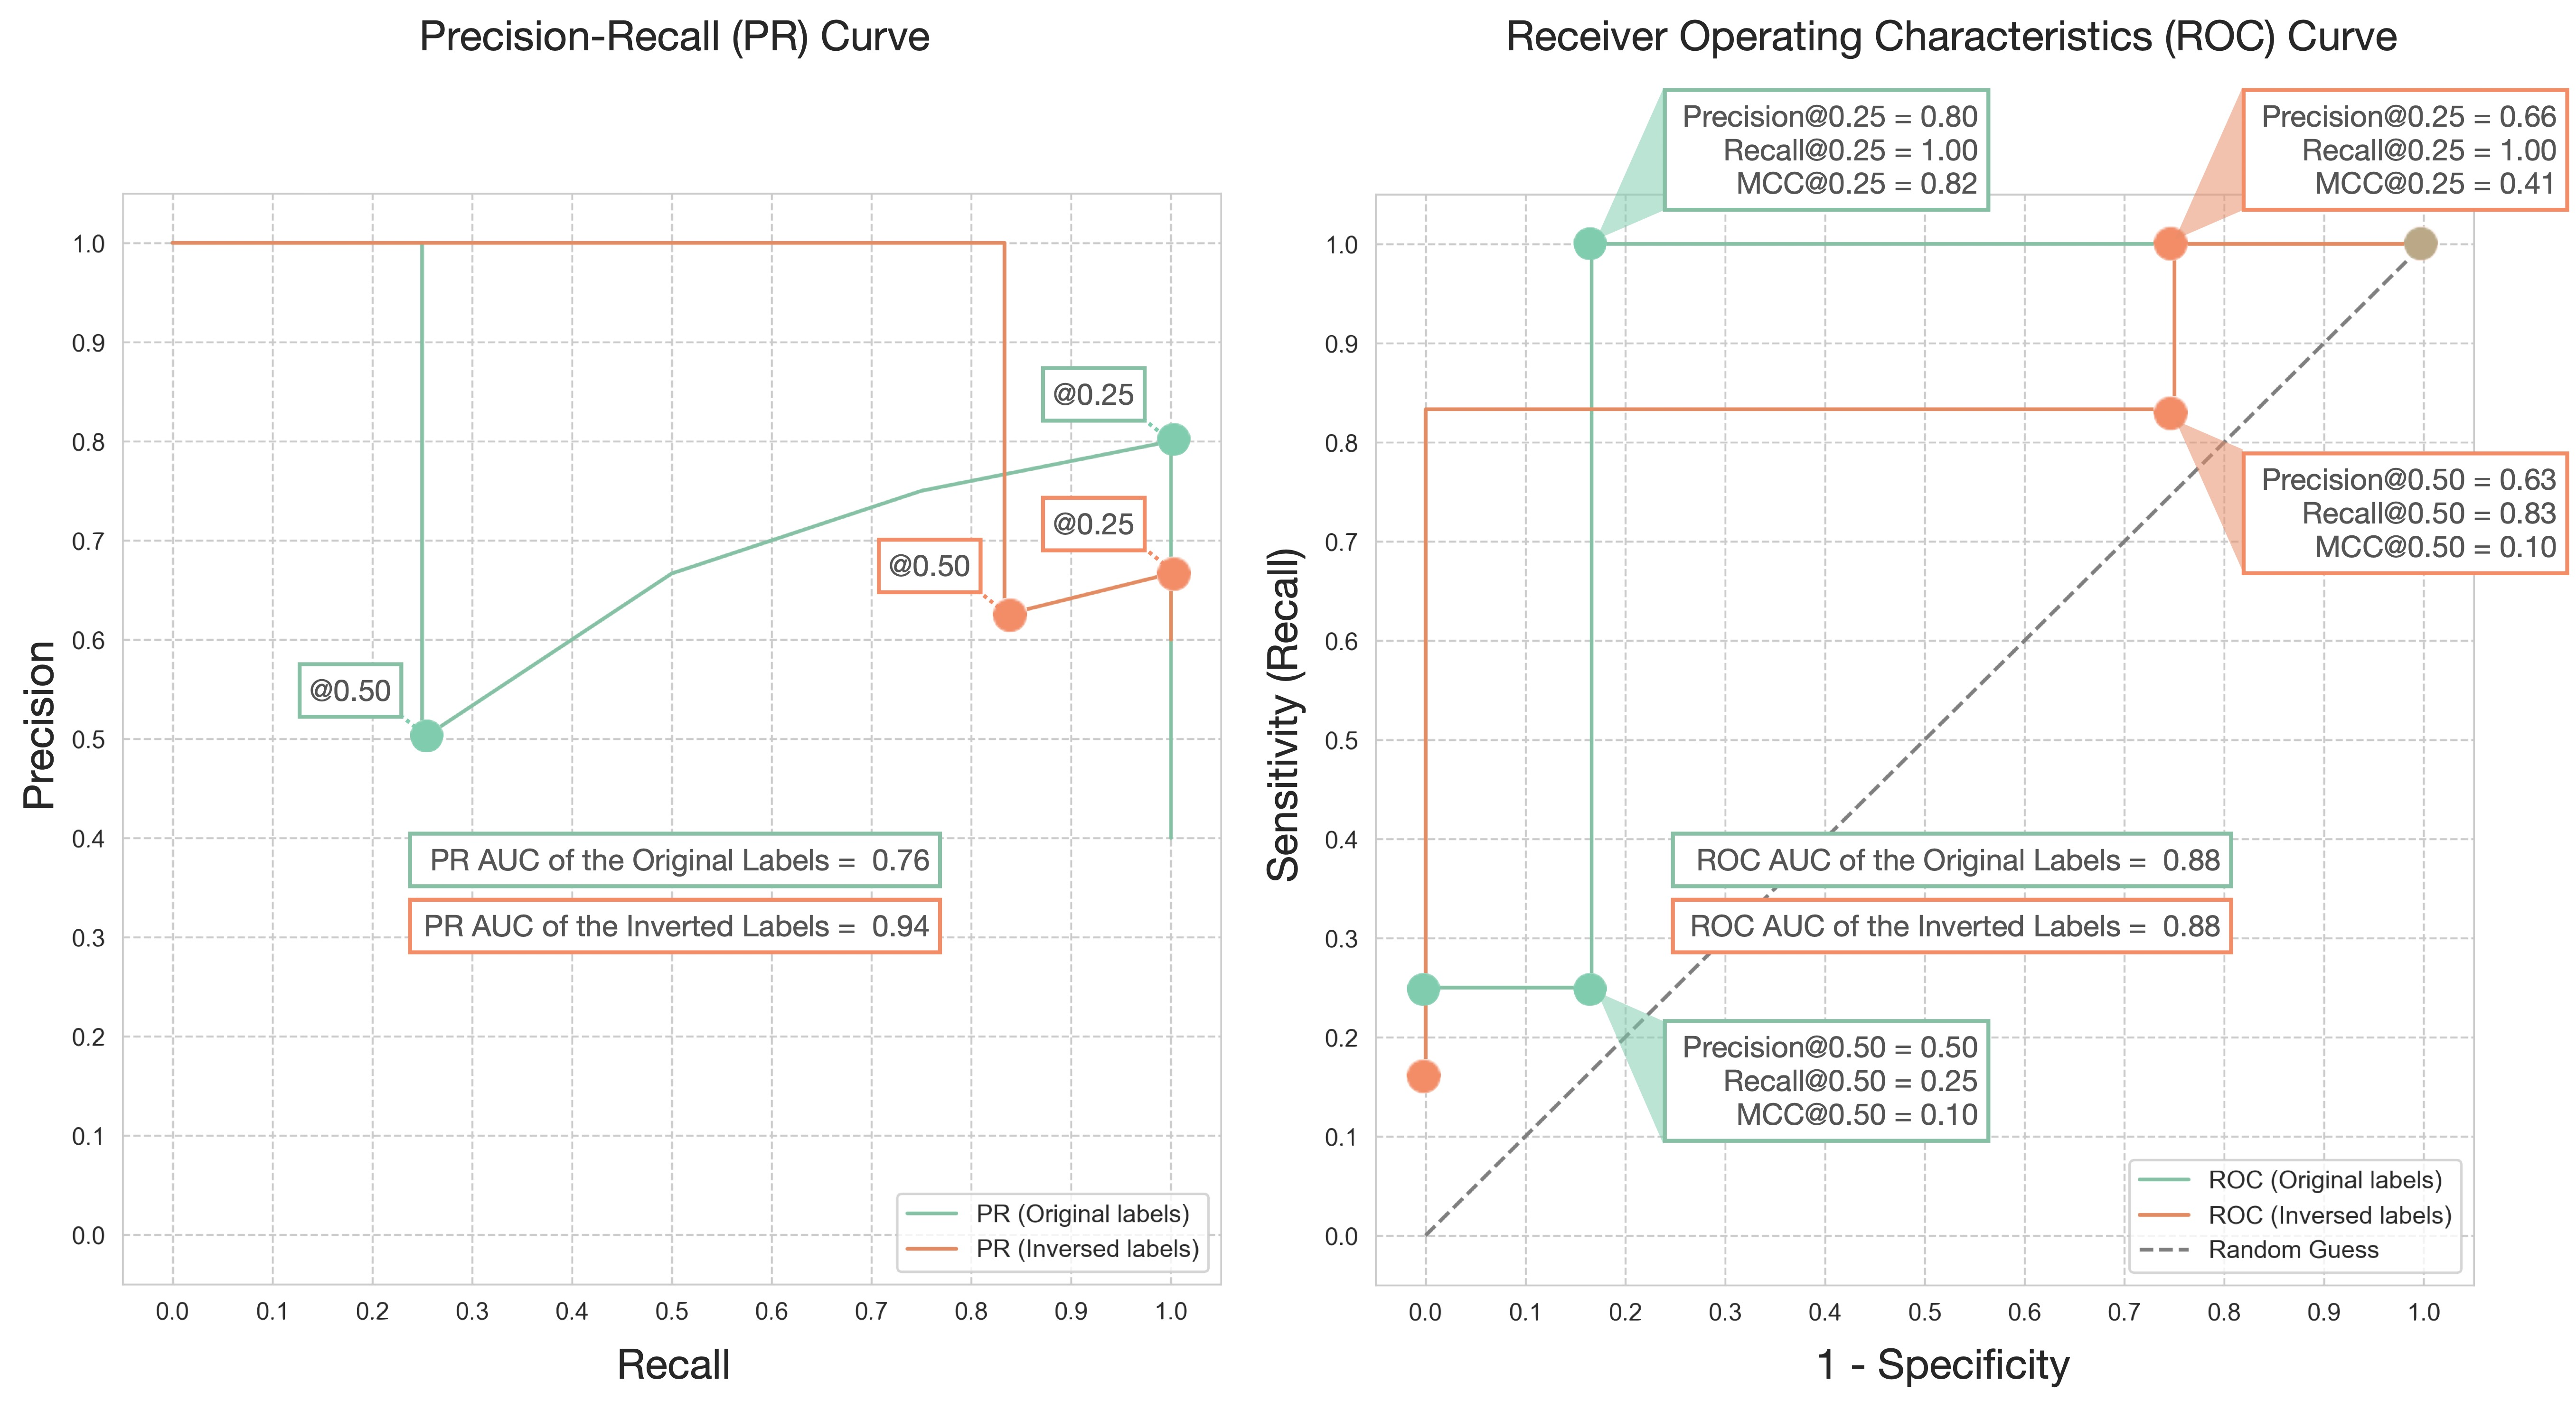
\includegraphics[width=1\textwidth]{fig_s5_curve.jpg}
    \caption{\textbf{(Left)} Precision-recall (PR) curve and \textbf{(Right)} Receiver operating characteristic (ROC) curve for the hypothetical example are displayed. The performance at confidence thresholds of 0.25 and 0.50 is highlighted. Original labels are marked in green, while inverted labels appear in orange. The Area Under the Curve (AUC) is depicted at the center of each curve.}
    \label{fig:s5_curve}
\end{figure}

However, it is worth re-emphasizing that precision and recall focus predominantly on positive samples. Inappropriately assigning a predominant background event as the positive class can lead to skewed interpretations. This pitfall is demonstrated in this example by inverting the labels. At a threshold of 0.50, precision increases from 0.50 to 0.63, and recall jumps from 0.25 to 0.83. With the threshold set at 0.25, precision drops to 0.66 from 0.80, while recall remains unchanged. The PR AUC also rises from 0.76 to 0.94. Such shifts in metrics, driven merely by label rearrangement unrelated to the data or model characteristics, underscore the importance of label-invariant metrics that remain unaffected by label assignments.
Unlike metrics focusing solely on positive samples, the ROC curve accounts for both positive and negative samples, making it a label-invariant metric. Specificity is plotted on the x-axis and sensitivity on the y-axis, calculated at different thresholds (Figure ~\ref{fig:s5_curve}, Right). In this hypothetical example, the ROC curve demonstrates robustness and label-invariance with a consistent AUC of 0.875, regardless of whether the original or inverted labels are used.
Lastly, another label-invariant metric is MCC which provides a balanced assessment of both positive and negative samples. Considering MCC's balanced approach to evaluating model performance, this study introduces the concept of an MCC curve. This curve, which plots the MCC value against various threshold levels (Figure ~\ref{fig:s5_mcc}), serves as a powerful tool for identifying the optimal confidence thresholds for model predictions. By examining this curve, one can determine the specific threshold at which the MCC value peaks, thereby optimizing the model's performance. For example, when applied to the hypothetical example, the optimum MCC value of 0.82 was attained at a threshold of 0.25. This particular threshold corresponded to accuracy, precision, and recall values of 0.90, 0.75, and 1.00, respectively. Notably, the MCC curve retains its symmetry even when labels are reversed, affirming its status as a label-invariant measure. In scenarios with inverted labels, the maximum MCC value observed was 0.83, achieved at a threshold of 0.75, leading to accuracy, precision, and recall values of 0.90, 1.00, and 0.83, respectively. Such findings underscore the MCC's ability to provide a balanced and comprehensive assessment of both positive and negative samples, thereby reinforcing its utility as a versatile and effective metric for thorough model evaluation.

In conclusion, binary classification models are often evaluated using metrics focusing on positive samples, such as precision and recall. It is generally advisable to designate the event of interest as the positive class. Otherwise, these metrics can be misleading when the more common but less significant background event is mistakenly marked as the positive class. To circumvent this potential bias, adopting label-invariant metrics is recommended. These metrics offer a more balanced and reliable assessment of model performance. Notable examples of such metrics include the ROC curve and the proposed MCC curve by this review, both of which are unaffected by the choice of positive and negative class labels and are thus robust for a thorough model evaluation.
\begin{figure}[h]
    \centering
    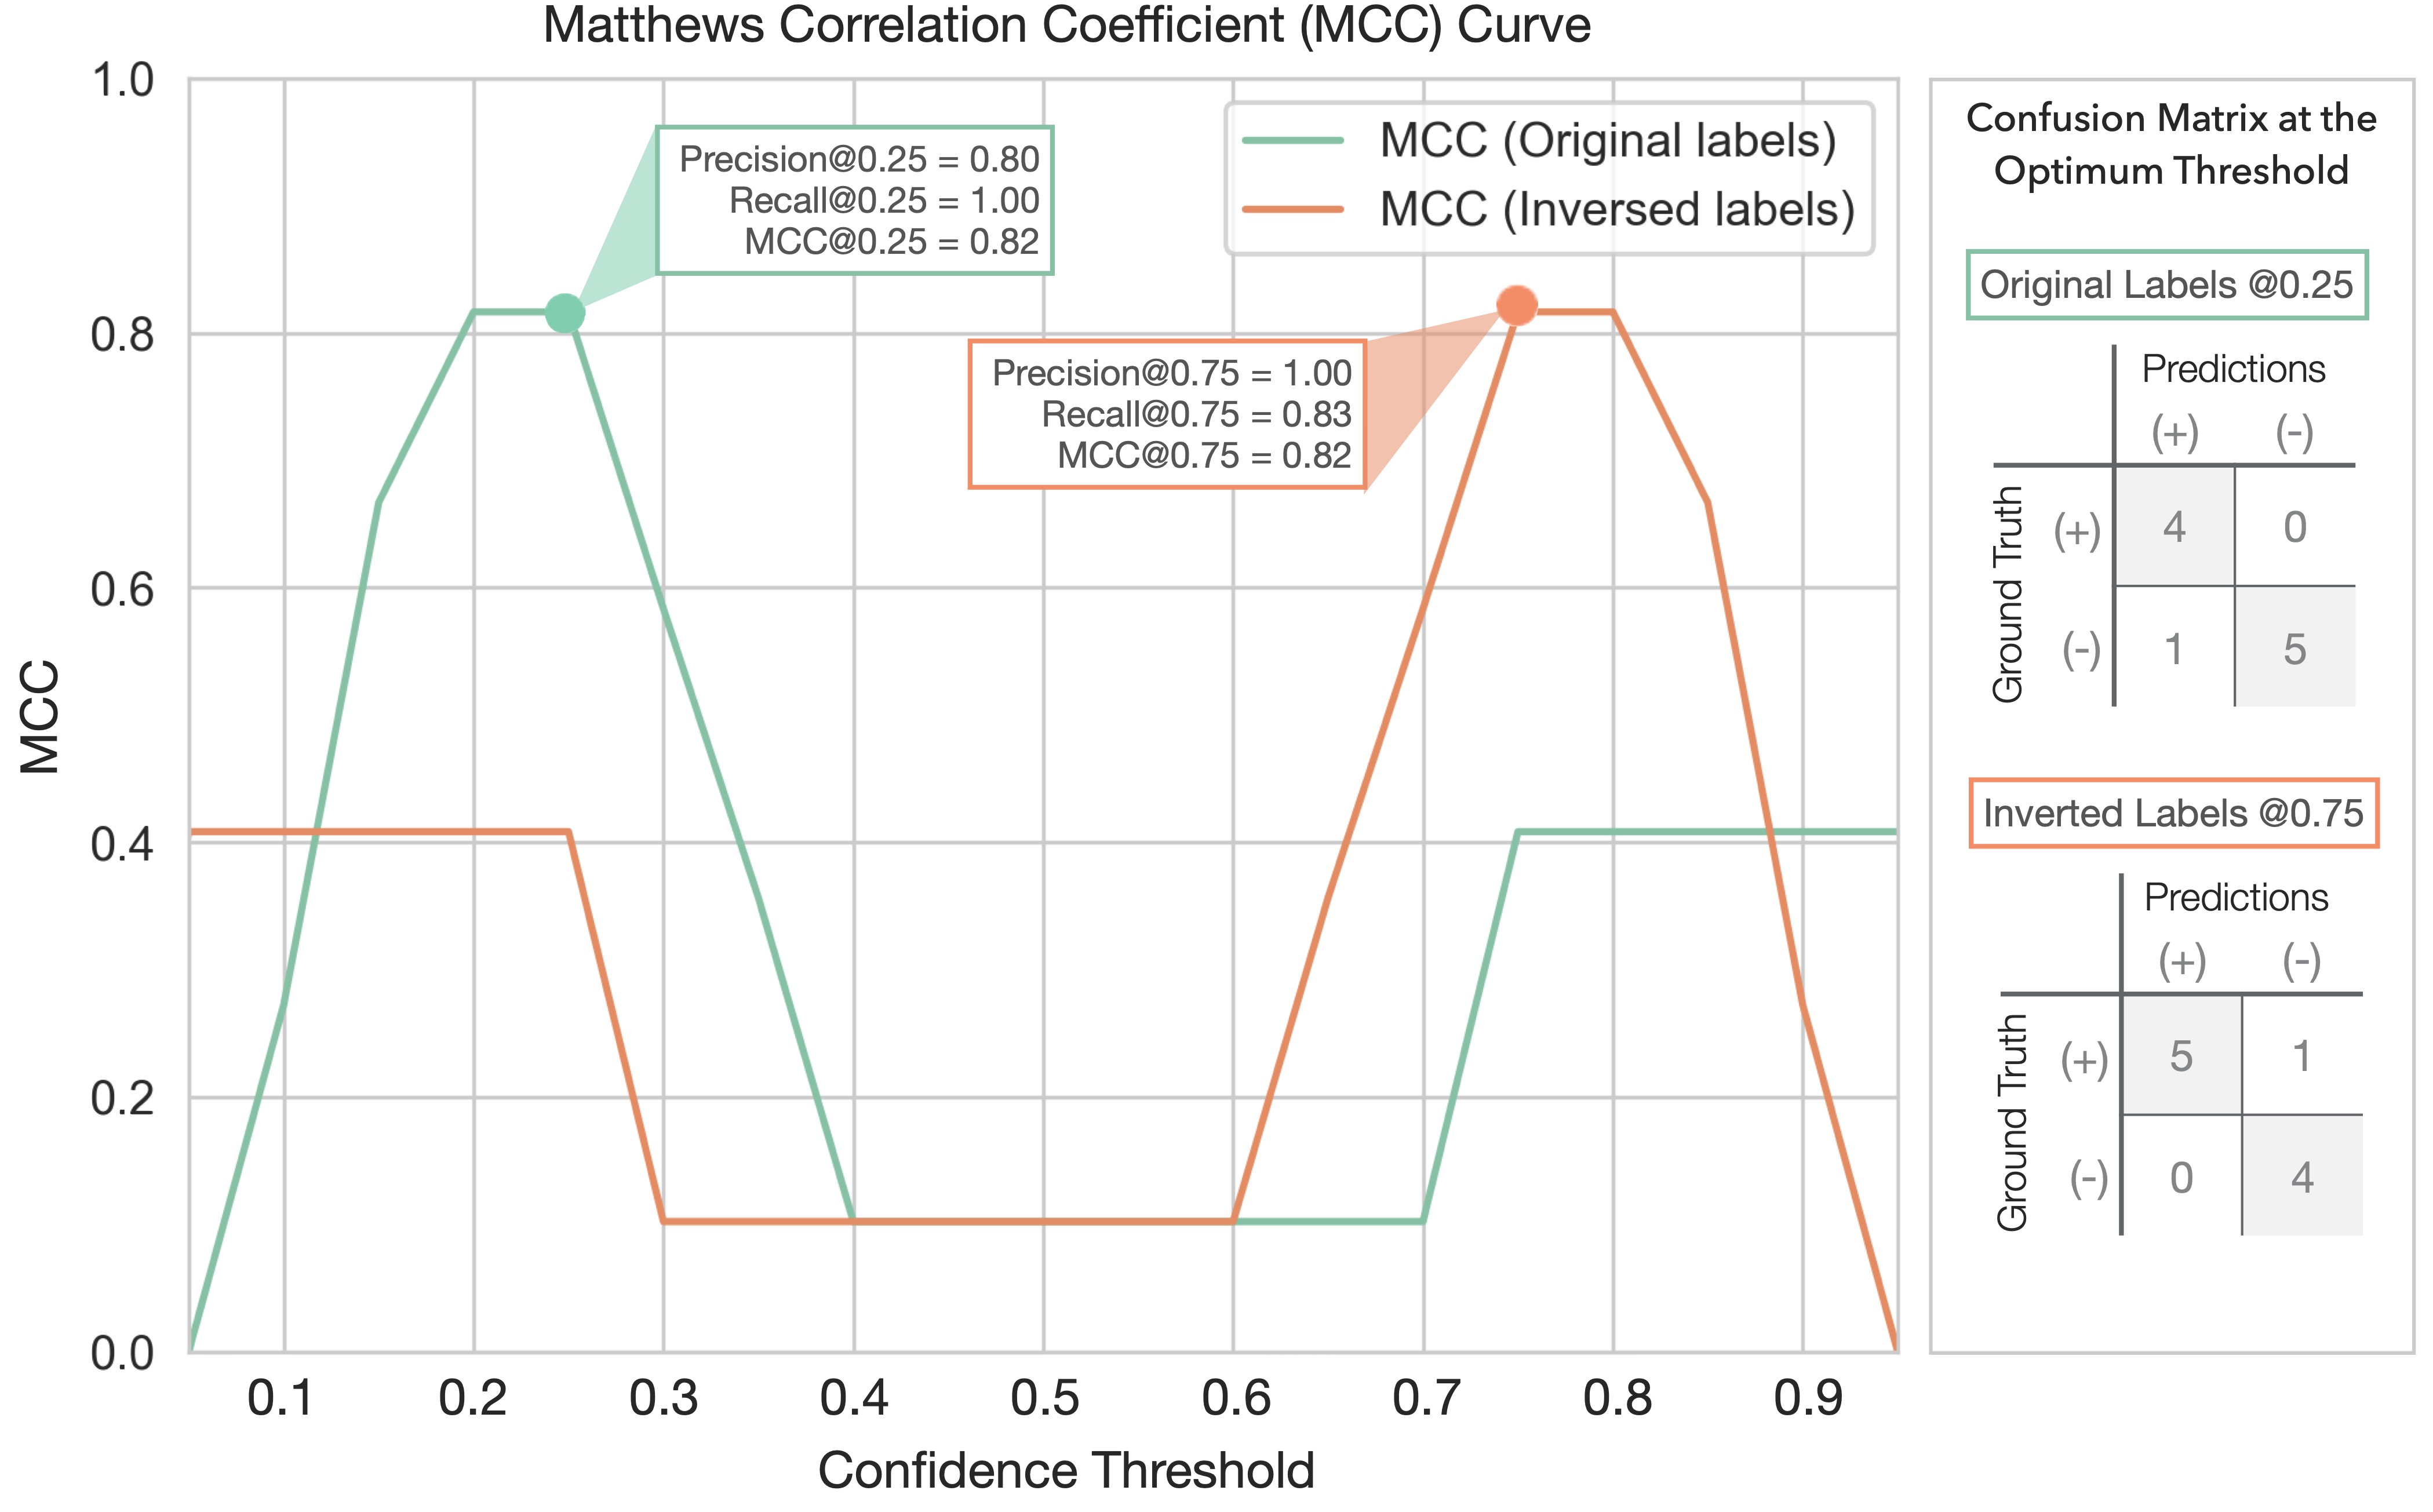
\includegraphics[width=.8\textwidth]{fig_s5_mcc.jpg}
    \caption{Matthews Correlation Coefficient (MCC) curve. A line chart plotting MCC at different thresholds for the hypothetical example. The optimal threshold is highlighted by the dot marks in green and orange for the original and inverted labels, respectively. The confusion matrix at the optimal threshold is displayed in the right panel.}
    \label{fig:s5_mcc}
\end{figure}